\section{Introduction}

\subsection{Motivation}
\frame{
  \frametitle{Visual SLAM Approaches}

  \begin{figure}[H]
    \begin{minipage}[r]{.15\textwidth}
      \caption{\footnotesize Sparse SLAM (PTAM, \cite{PTAM})}
    \end{minipage}  
    \begin{minipage}[c]{.2\textwidth}
      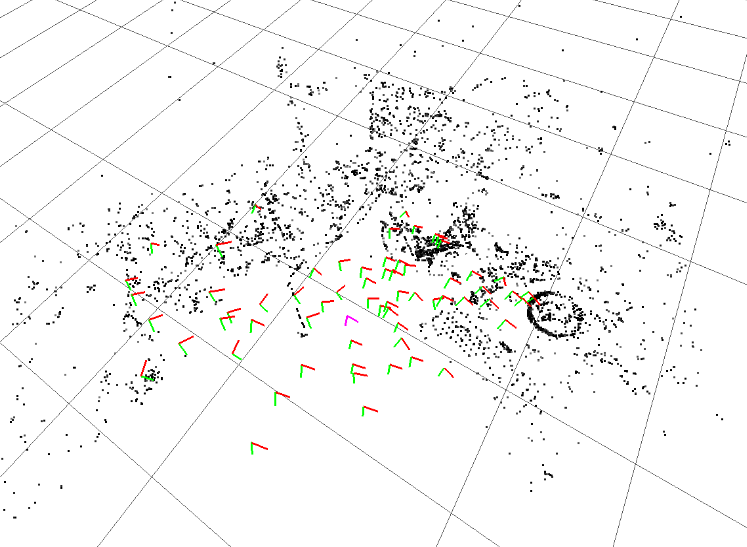
\includegraphics[width=\linewidth]{figures/sparse.png}
    \end{minipage}
    \hspace{2em}
    \begin{minipage}[c]{.2\textwidth}
      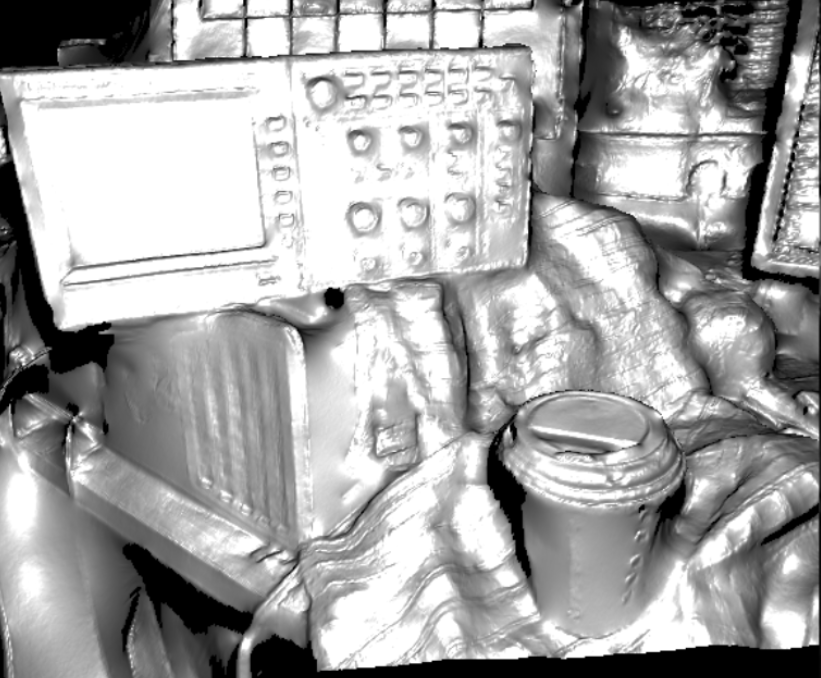
\includegraphics[width=\linewidth]{figures/DTAM.png}
    \end{minipage}
    \begin{minipage}[l]{.15\textwidth}
      \caption{\footnotesize Dense SLAM (DTAM, \cite{DTAM})}
    \end{minipage}  
    \\
    \vspace{1em}
    \begin{minipage}[c]{.25\textwidth}
      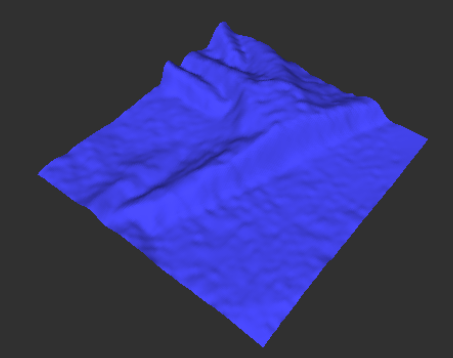
\includegraphics[width=\linewidth]{figures/Dominik.png}
      \centering
    \end{minipage}
    \begin{minipage}[l]{.15\textwidth}
      \caption{\footnotesize Dense SLAM with B-Splines \cite{Dominik}}
    \end{minipage}  
  \end{figure}

  \imp{$\implies$ Choice: Dense SLAM with B-Splines}

    % \begin{subfigure}{.3\linewidth}
      % 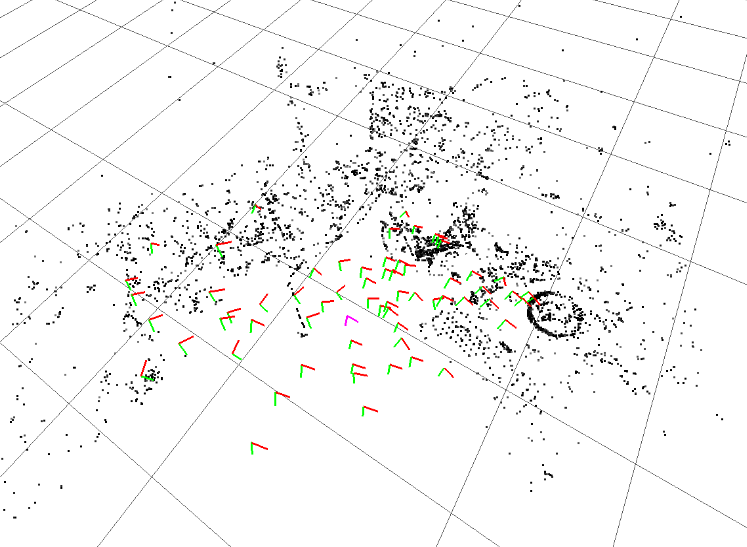
\includegraphics[width=\linewidth]{figures/sparse.png}
        % \caption{\footnotesize Sparse SLAM (PTAM, \cite{PTAM})}
      % \end{subfigure}
    % \begin{subfigure}{.3\linewidth}
        % 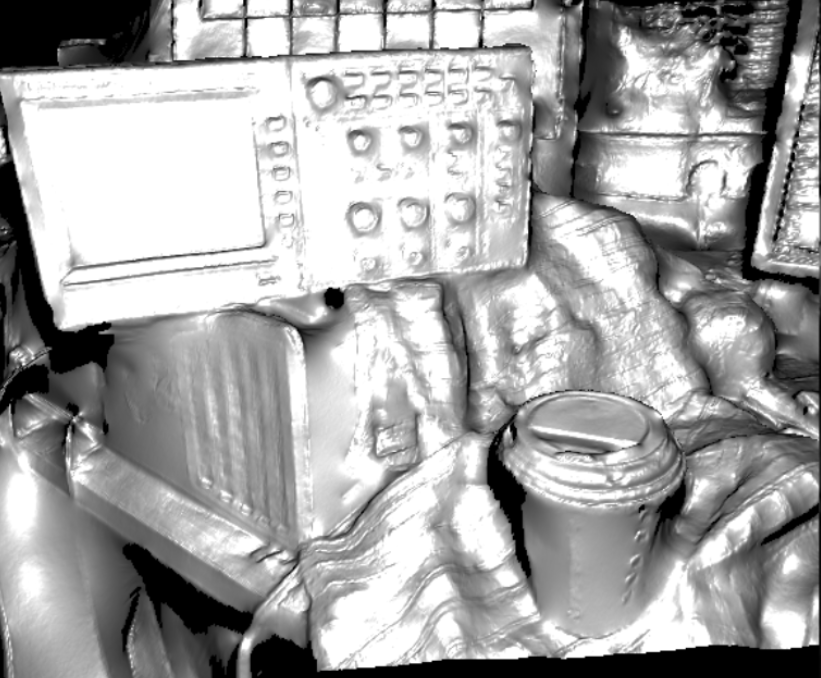
\includegraphics[width=\linewidth]{figures/DTAM.png}}
        % \caption{Dense SLAM (DTAM, \cite{DTAM})
    % \end{subfigure} 
    % \begin{subfigure}{.3\linewidth}
      % 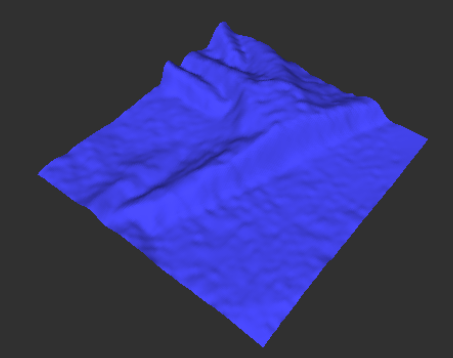
\includegraphics[width=\linewidth]{figures/Dominik.png}
        % \caption{\footnotesize Dense SLAM with Splines (ASL, \cite{Dominik})}
    % \end{subfigure}
  % \end{figure}
}

\subsection{Project Goals}
\frame{
  \frametitle{Visual Terrain Estimation For Legged Robots}

  \imp{Framework for dense stereo camera SLAM }

  \begin{itemize}
      \item Static stereo camera $\implies$ spline surface (map)
      \item Map $\implies$ new camera position
    \end{itemize}

  \begin{figure}[H]
    \centering
    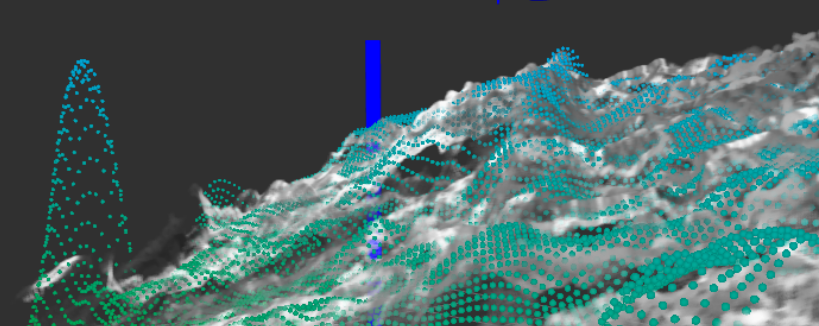
\includegraphics[width=.7\linewidth]{figures/goal.png}
  \end{figure}
  }

    
\subsection{Methods}
% \frame{
  % \frametitle{Visual Terrain Estimation For Legged Robots}
  % \begin{itemize}
      % \item \textbf{Simulation environment}: \ros with \rviz for pointcloud and
      % \opencv for image handling.
    % \item \textbf{Optimization}: own implementation of optimization algorithm using \eigen 's sparse matrix solvers.
    % \item \textbf{Hardware}: \rovio sensor for stereo camera data,
      % \textit{MacBook Pro} with Intel Core 2.7MHz, 4 cores.
  % \end{itemize}
% }
